\chapter[Cronograma]{Cronograma}
\label{chap:crono}

A Figura \ref{img:cronograma} mostra o cronograma das atividades realizadas durante a primeira parte do projeto.

\begin{figure}[H]
    \centering
    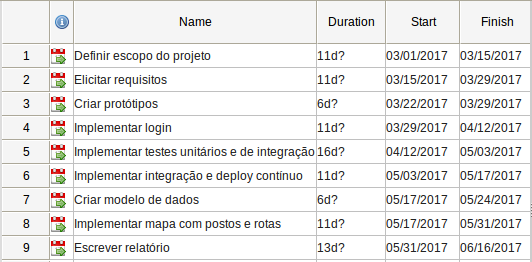
\includegraphics[scale=0.5]{figuras/cronograma_r1.png}
    \caption[Cronograma de atividades da primeira entrega.]{Cronograma de atividades da primeira entrega. Fonte: autores}
    \label{img:cronograma}
\end{figure}

Na Figura \ref{img:cronograma2inicial} tem-se o cronograma inicial da segunda parte do projeto.

\begin{figure}[H]
    \centering
    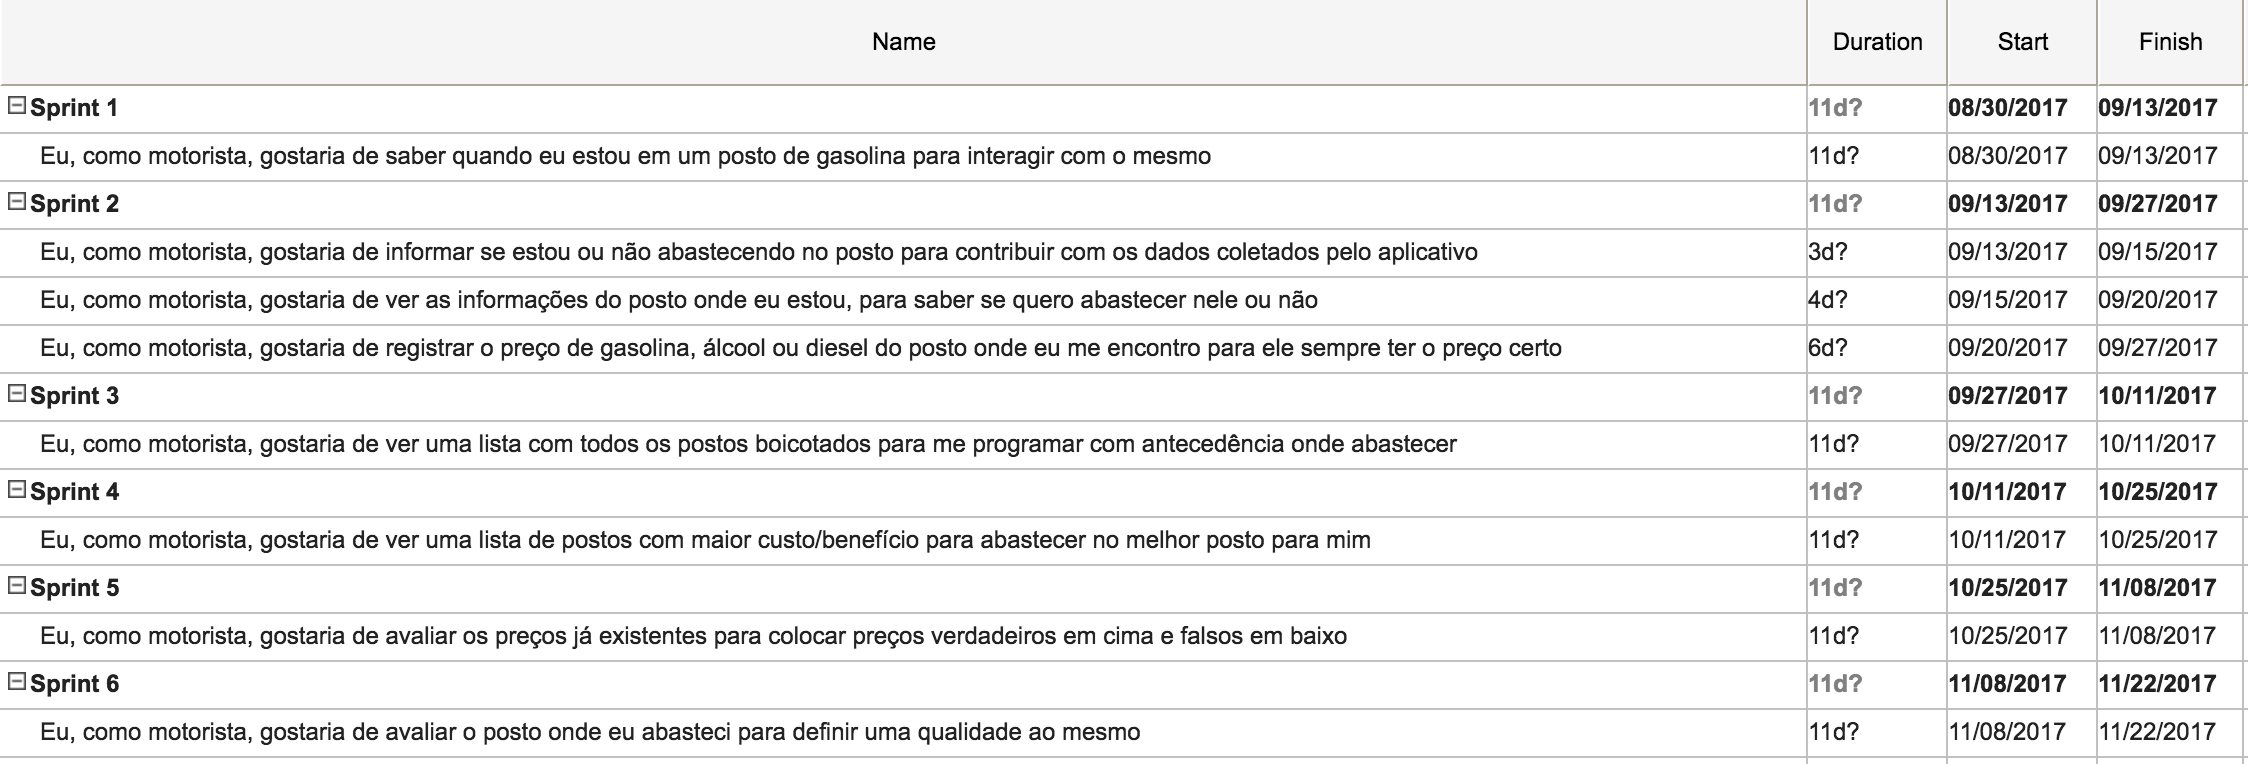
\includegraphics[scale=0.4]{figuras/cronograma_segunda_parte_1.png}
    \caption[Cronograma inicial de atividades da segunda entrega.]{Cronograma inicial de atividades da segunda entrega. Fonte: autores}
    \label{img:cronograma2inicial}
\end{figure}
\pagebreak

Porém, devido a certas adversidades e melhor compreensão do projeto, foram feitas certas mudanças no cronograma como mostra a Figura \ref{img:cronogramafinal}.

\begin{figure}[H]
    \centering
    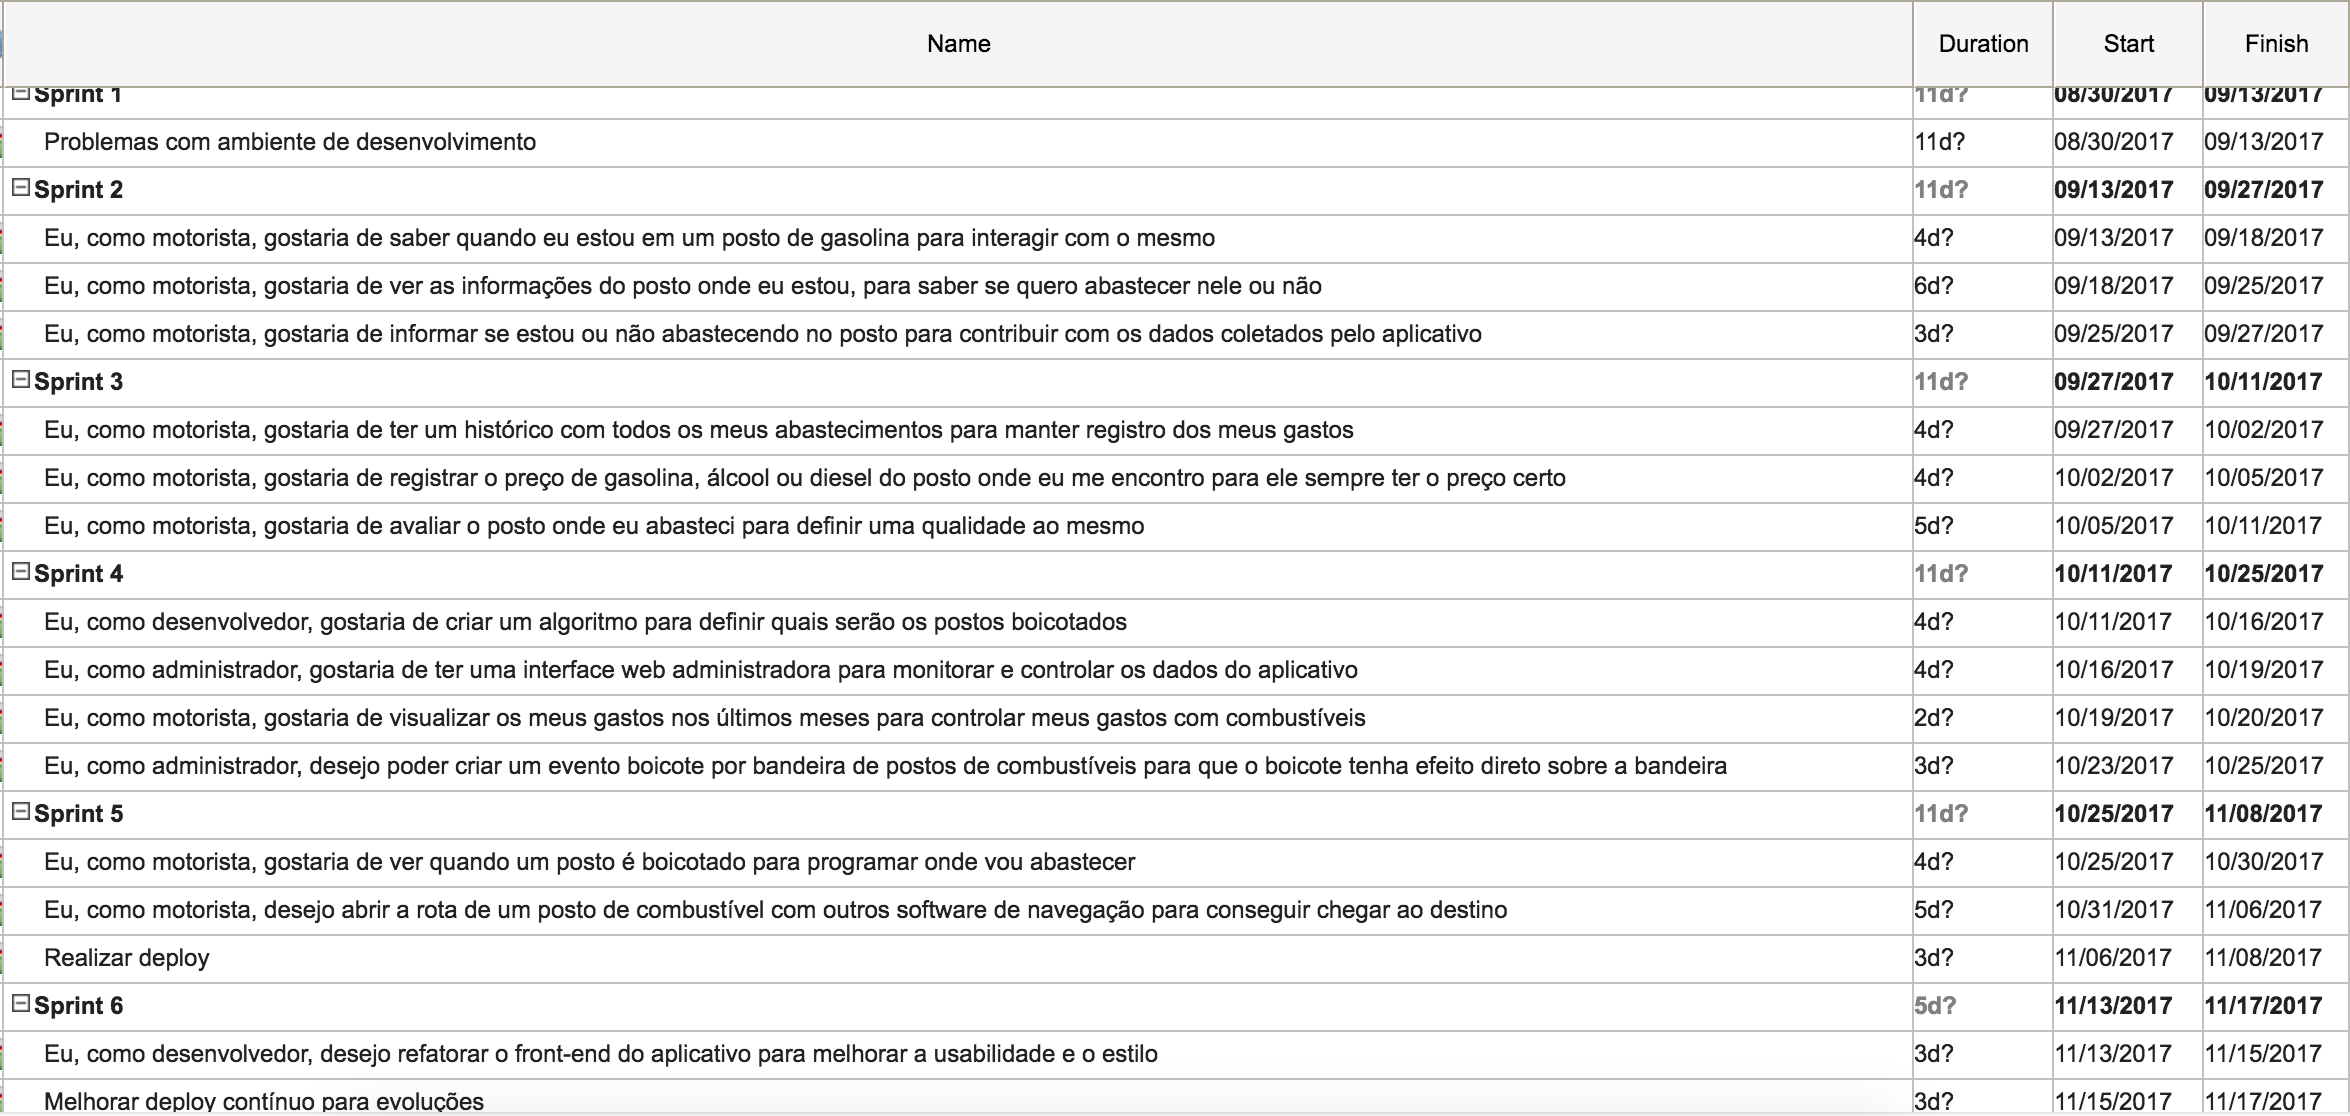
\includegraphics[scale=0.4]{figuras/cronograma_segunda_parte_2.png}
    \caption[Cronograma final de atividades da segunda entrega.]{Cronograma final de atividades da segunda entrega. Fonte: autores}
    \label{img:cronogramafinal}
\end{figure}

Principalmente na primeira \textit{sprint}, problemas foram encontrados com o ambiente de desenvolvimento do Ionic por causa da atualização do Ionic 2 para o Ionic 3. A maioria dos problemas relacionados com atualizações de dependências.

O \textit{plugin} do \textit{Geofence}, utilizado para definir cercas geográficas nos postos para indicar ao usuário quando ele entra em um posto de combustíveis, é implementado para o iOS na linguagem de programação Swift. A Apple, atualizou o Swift da versão 2 para a versão 3 durante o desenvolvimento, e o plugin não foi atualizado ainda. Ocasionando incompatibilidade do serviço oferecido pelo \textit{plugin} com a plataforma iOS. Mesmo depois de muitas tentativas de fazê-lo funcionar nesta plataforma, não foi obtido êxito, levando com que a equipe de desenvolvimento juntamente com o professor orientador tomassem a decisão de pausar o desenvolvimento para a plataforma iOS e focar apenas para o Android, evitando assim que todo o trabalho fosse prejudicado pela atualização de uma dependência que ainda não ocorreu.

Além do problema da plataforma da Apple, apesar do \textit{plugin} \textit{Geofence} ter suporte para notificações \textit{push} (mensagens de alerta enviadas para o usuário notificando na tela do aparelho) locais, uma opção para facilitar a escalabilidade do aplicativo, caso for preciso enviar notificações \textit{push} em outros momentos, foi a utilização de algum serviço externo para enviar as notificações. Por causa dessa decisão, a impelementação da funcionalidade acabou atrasando mais do que devia, pois foi necessário realizar pesquisas sobre novas alternativas. Por fim, foi utilizado o serviço de notificações \textit{push} da Google, o Firebase.

Durante a sprint 4, percebeu-se que seria necessário uma tela de administração para poder definir os ícones dos postos assim como corrigir quaisquer informações incorretas vindo das fontes externas e por isso foi adicionado no cronograma. Durante a mesma sprint, viu-se necessário melhorar a inteface do aplicativo pois o foco até então foi exclusivamente em desenvolver as funcionalidades. Porém, esse melhoria foi alocada para a sprint 6 porque a sprint 4 e a sprint 5 já possuiam muitas tarefas.
